\part{Data representation}
\frame{\partpage}

\begin{frame}{Memory}
	\pause
	\begin{center}
		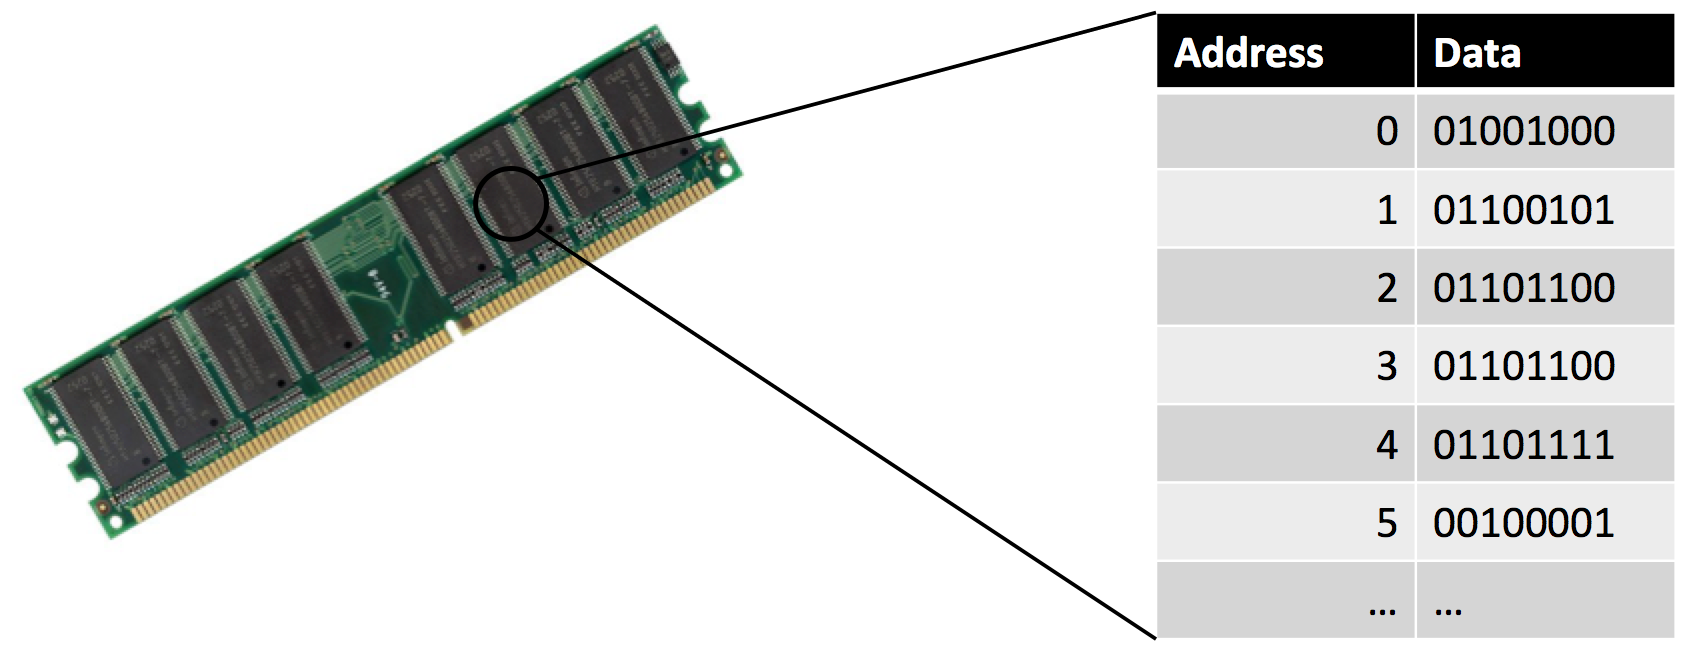
\includegraphics[width=0.8\textwidth]{memory}
	\end{center}
	\begin{itemize}
		\item Memory works like a set of \textbf{boxes}
		\pause\item Each box has a number, its \textbf{address}
		\pause\item Each box contains a \textbf{byte} (8 bits)
	\end{itemize}
\end{frame}

\begin{frame}{Data representation} 
	\begin{itemize}
		\pause\item All data is stored as \textbf{sequences of bytes}
			\begin{itemize}
				\pause\item Sequence of bits, in multiples of 8
				\pause\item Sequence of numbers between 0--255
			\end{itemize}
	\end{itemize}
\end{frame}

\begin{frame}{Number bases}
	\begin{itemize}
		\pause\item Decimal = base 10
		\pause\item Binary = base 2
		\pause\item Octal = base 8
		\pause\item Hexadecimal = base 16
			\begin{itemize}
				\pause\item Uses \texttt{A}--\texttt{F} as extra ``digits''
			\end{itemize}
		\pause\item We sometimes write the base as a \textbf{subscript}
			\begin{itemize}
				\pause\item $123_{10} = 7B_{16} = 173_{8} = 01111011_{2}$
			\end{itemize}
	\end{itemize}
\end{frame}

\begin{frame}[fragile]{Number bases in code}
	\begin{itemize}
		\pause\item In most languages (including C, C++, C\#, Python):
			\begin{itemize}
				\pause\item Decimal: \texttt{123}
				\pause\item Binary: \texttt{0b1111011}
				\pause\item Hexadecimal: \texttt{0x7B}
			\end{itemize}
		\pause\item In some languages (including C, C++, Python 2.x):
			\begin{itemize}
				\pause\item Octal: \texttt{0173}
			\end{itemize}
		\pause\item So beware of leading zeroes!
	\end{itemize}
	\begin{lstlisting}
>>> print 77
77
>>> print 077
63
	\end{lstlisting}
\end{frame}

\begin{frame}{Why is hexadecimal useful?} 
	\begin{itemize}
		\pause\item It is easy to convert between binary and hexadecimal
		\pause\item One hex digit = 4 bits
	\end{itemize}
	
	\pause $$
	\underbrace{0001}_{1}
	\underbrace{1110}_{E}
	\underbrace{0010}_{2}
	\underbrace{0100}_{4}
	\underbrace{0000}_{0}
	$$
	
	\pause So $1\,1110\,0010\,0100\,0000_{2} = 1E240_{16}$
\end{frame}

{
\setbeamercolor{background canvas}{bg=white}
\begin{frame}[plain]
	\begin{tikzpicture}[remember picture, overlay]
		\node[at=(current page.center)] {
			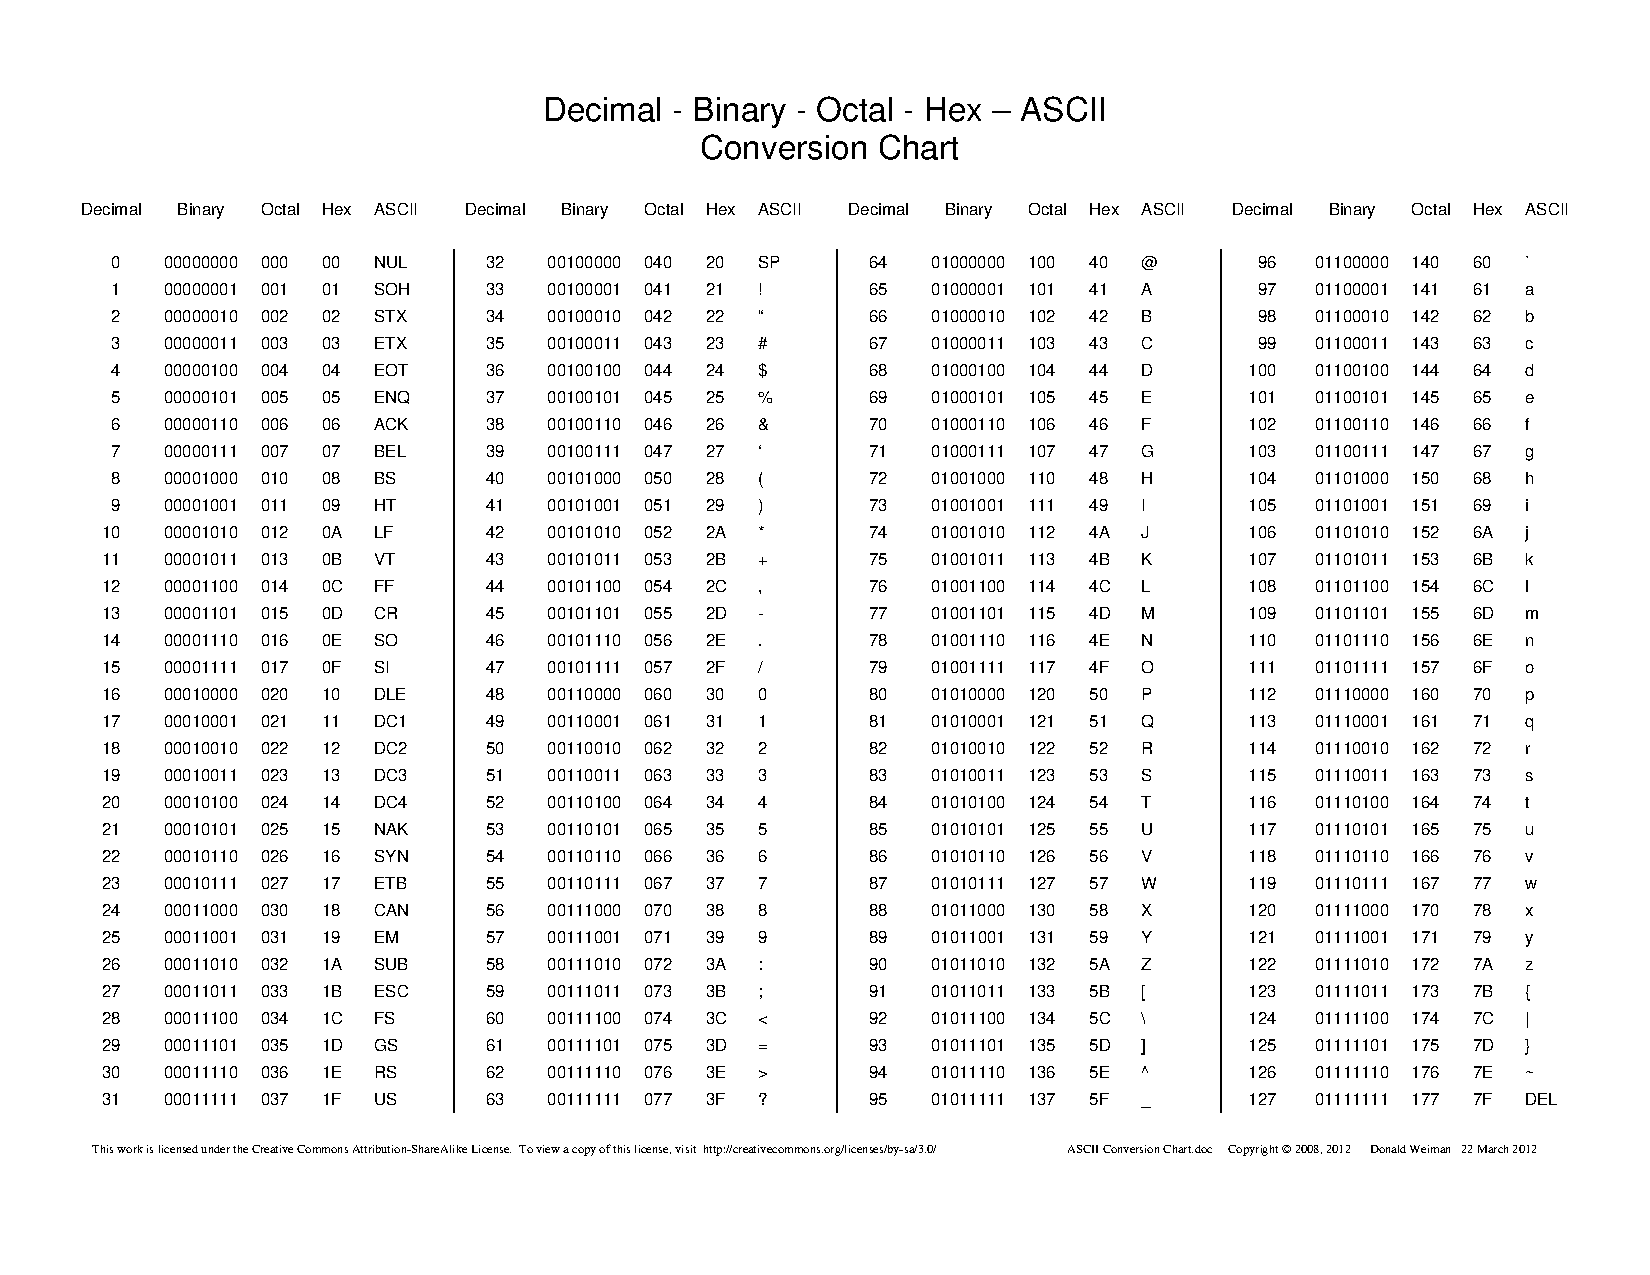
\includegraphics[width=\paperwidth]{ascii_chart}
		};
	\end{tikzpicture}
\end{frame}
}

\begin{frame}{Integers} 
	\begin{itemize}
		\pause\item Represented in \textbf{binary}
		\pause\item $n$ bits $\implies$ numbers from $0$ to $2^n-1$ inclusive
	\end{itemize}
\end{frame}

\begin{frame}{Endian-ness}
	\begin{itemize}
		\pause\item Intel x86/x64 architecture is \textbf{little endian}
		\pause\item Bytes are in ``reverse'' order (least significant first)
		\pause\item E.g.\ $123456_{10} = 1E240_{16}$, represented as
			\texttt{40 E2 01 00}
	\end{itemize}
\end{frame}

